\subsection{Interplay between parameters and FLOPs per example}
\label{app:n_s_d_interaction}

Recall that in~\Cref{sec:n_s_d_interaction}, we showed that isoFLOP curves were predictive of pretraining loss for different parameter counts and sparsity levels.
In this section, we show similar results with additional training compute budgets.
\begin{enumerate}[left=0pt,itemsep=2pt]
    \item In~\Cref{fig:additional_surfaces}, we first show that IsoFLOP surfaces mapping model size $N$ and sparsity level $S$ to pre-training loss $L$ are predictive in a similar way for all training compute budgets that we consider, ranging from 3e19 to 1e21 FLOPs. 
    \item In~\Cref{fig:additional_surface_eval}, we analyze the fitted IsoFLOP surfaces (one for each training budget) and find that the (a) effect of model size $N$ on optimal \moe sparsity $S^*$ and (b) the effect of \moe sparsity $S$ on the optimal total and active parameters, $N*$ and $N^*_a$, is similar for all training budgets.
\end{enumerate}

\begin{figure}[bp]
    \centering
    \subfigure{%{\textwidth}
        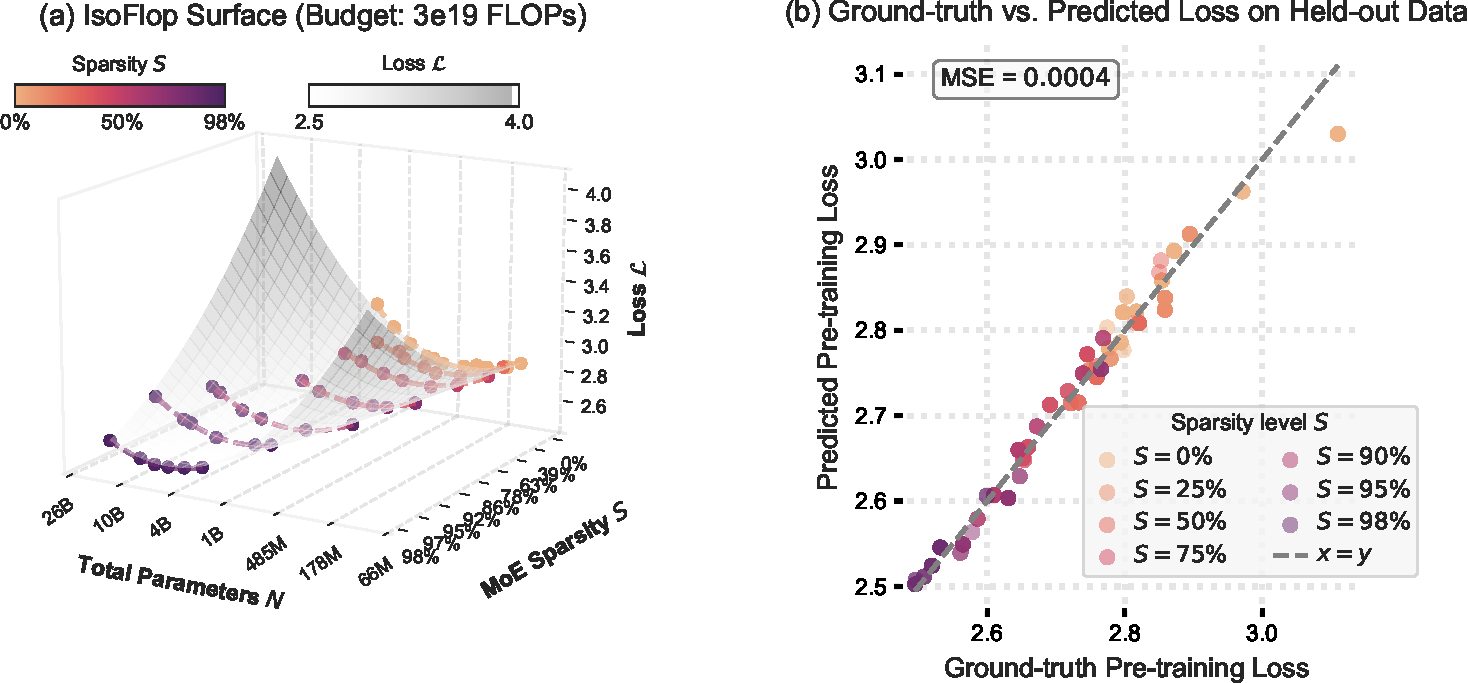
\includegraphics[width=0.45\textwidth]{plots/appendix/app_s2_3e19.pdf}
        \label{fig:isoflop_surface_3e19}
}
\subfigure{%{\textwidth}
        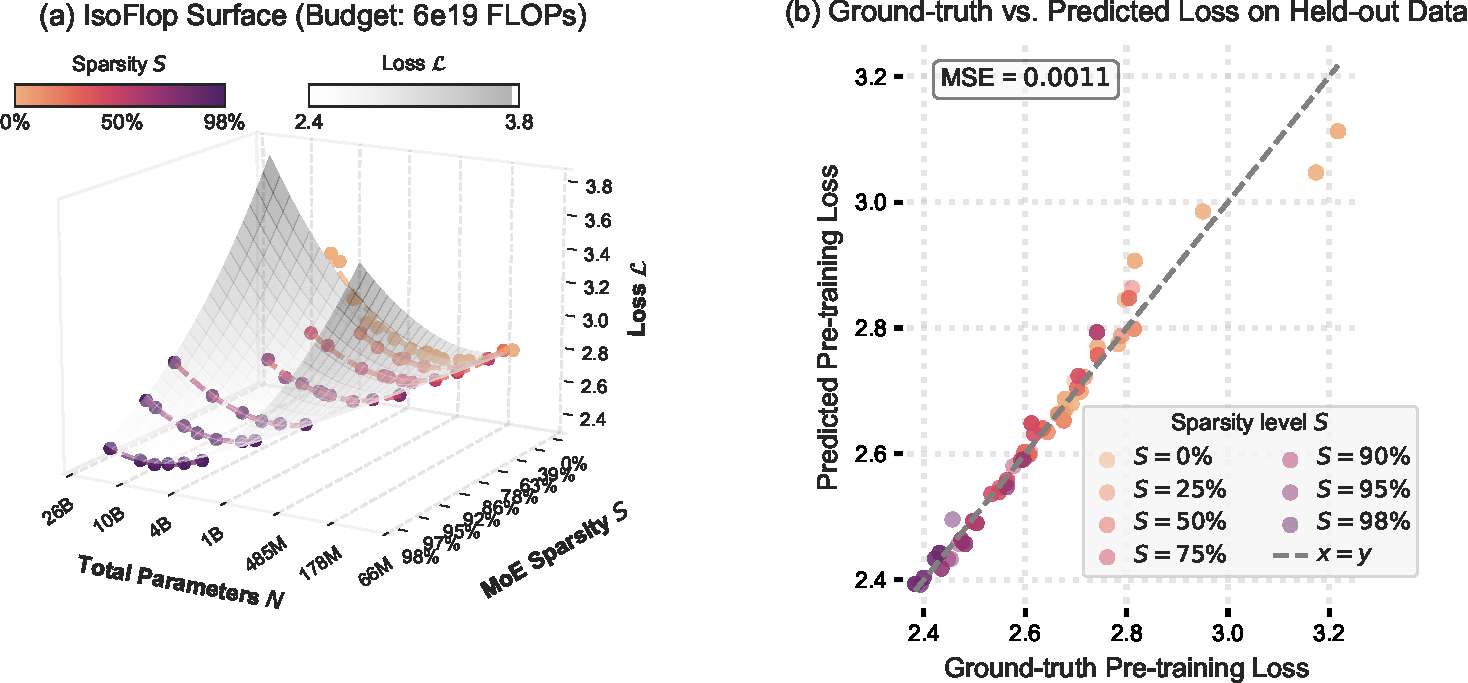
\includegraphics[width=0.45\textwidth]{plots/appendix/app_s2_6e19.pdf}
        \label{fig:isoflop_surface_6e19}
}
\subfigure{%{\textwidth}
        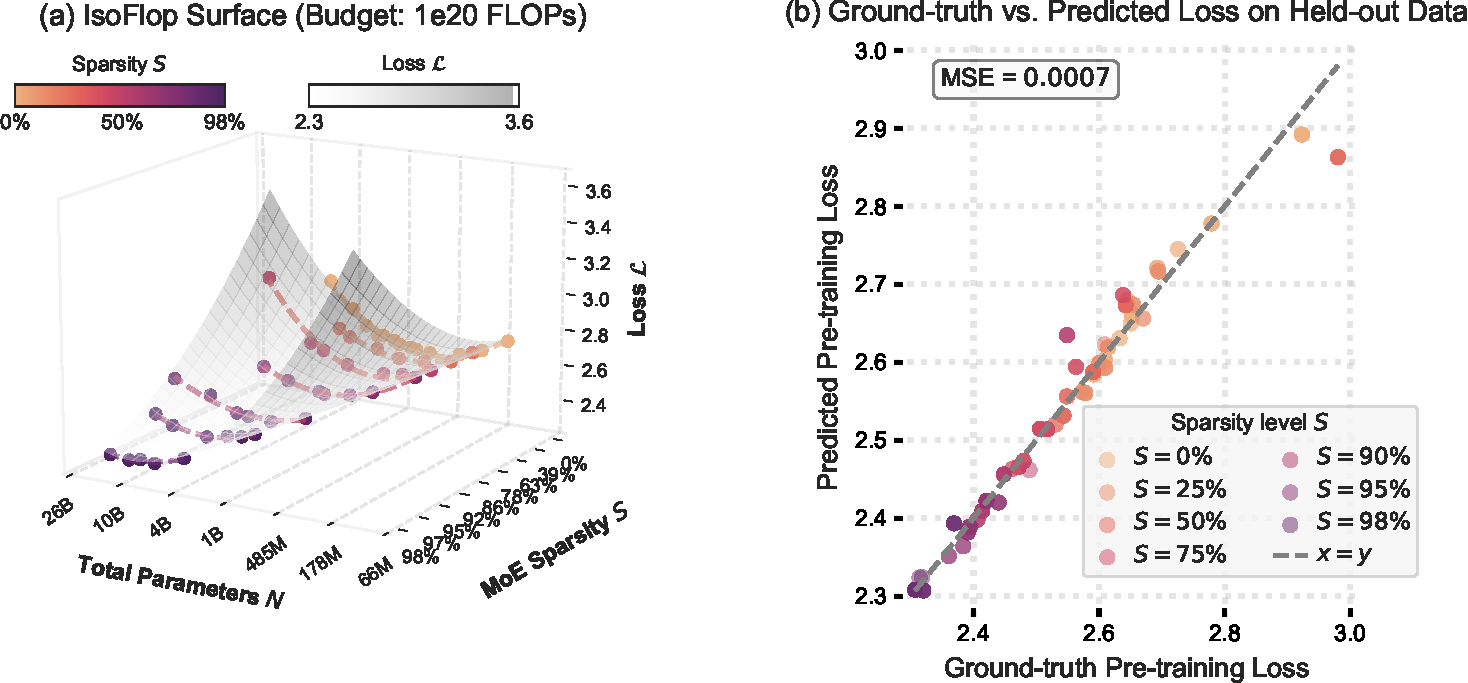
\includegraphics[width=0.45\textwidth]{plots/appendix/app_s2_1e20.pdf}
        \label{fig:isoflop_surface_1e20}
}
\subfigure{%{\textwidth}
        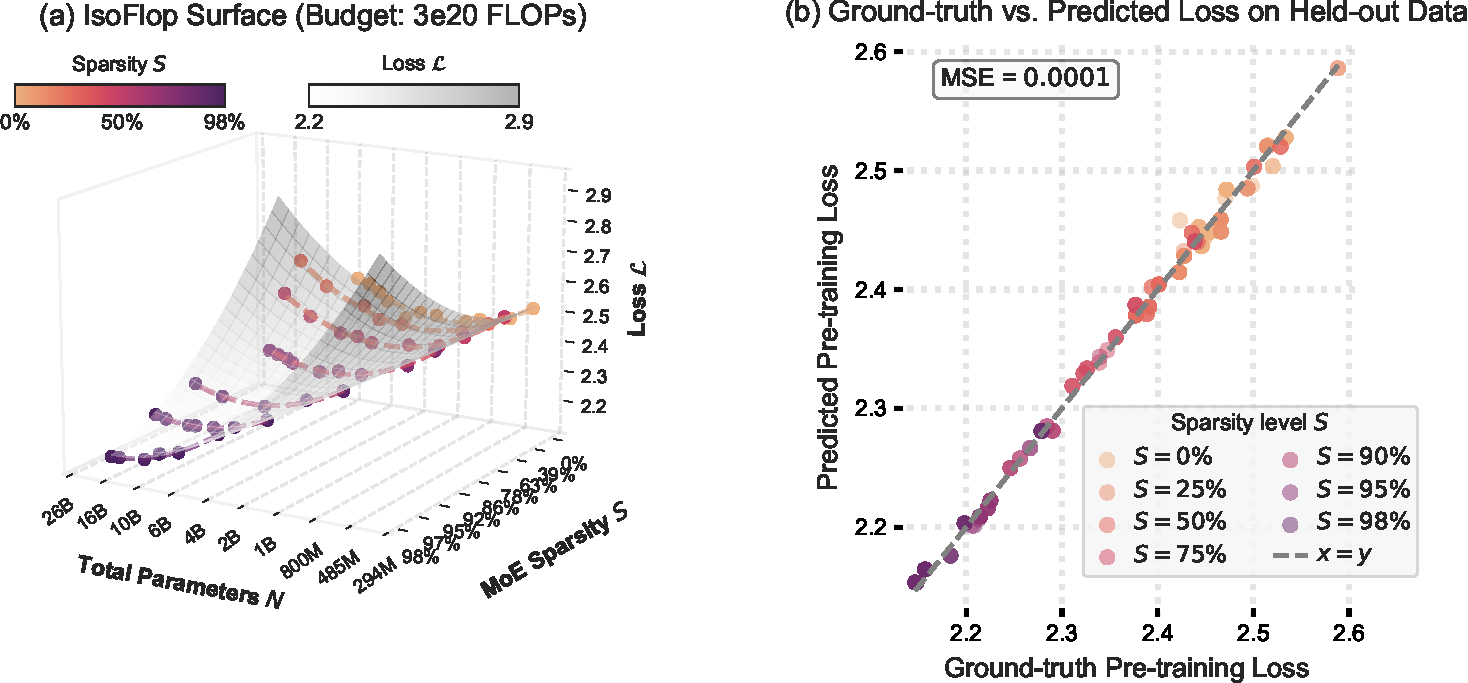
\includegraphics[width=0.45\textwidth]{plots/appendix/app_s2_3e20.pdf}
        \label{fig:isoflop_surface_3e20}
}
\subfigure{%{\textwidth}
        \centering
        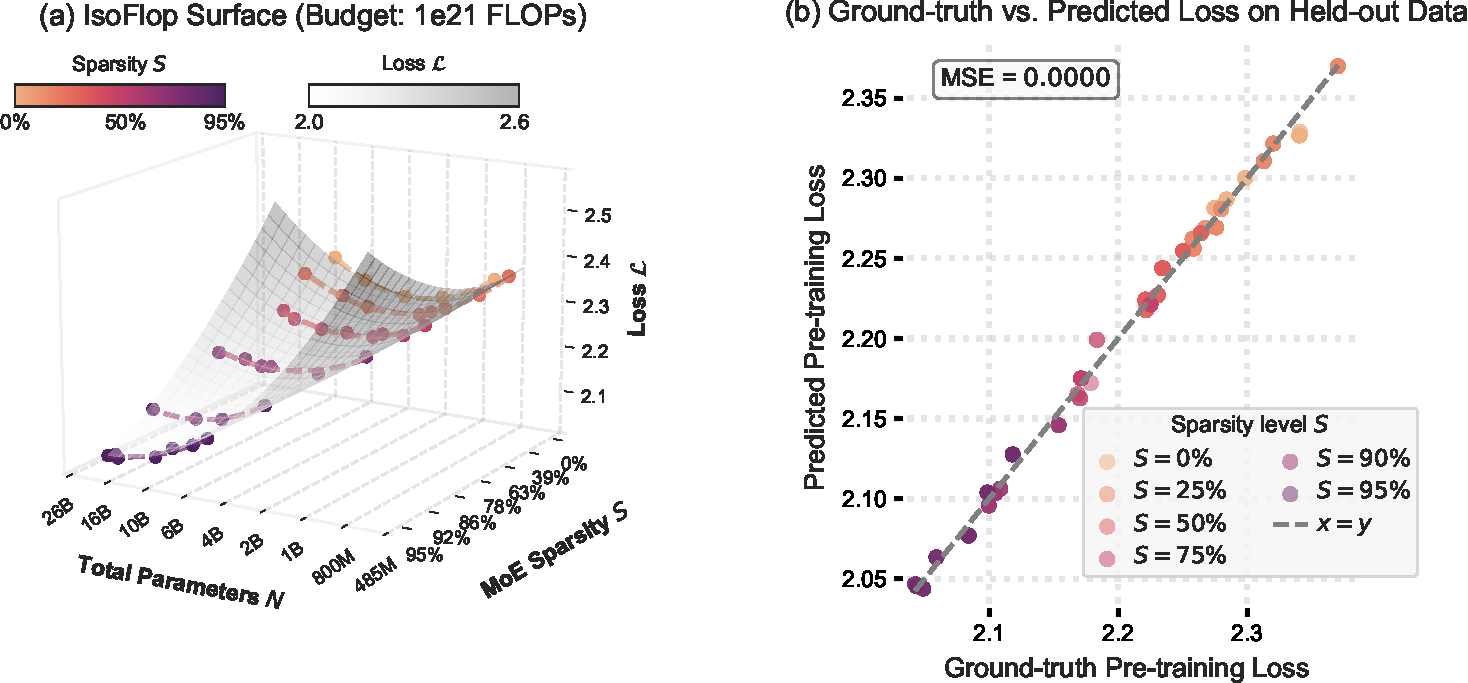
\includegraphics[width=0.45\textwidth]{plots/appendix/app_s2_1e21.pdf}
        \label{fig:s2_sub5}
}
    \caption{
        \textbf{IsoFLOP surfaces over total parameters $N$, \moe sparsity $S$, and pretraining loss $L$ for different compute budgets}. 
        The rows correspond to IsoFLOP surface fitted using models trained with a budget of 3e19, 6e19, 1e20, 3e20, and 1e21.  
        The subplots on the left visualize IsoFLOP surfaces mapping total parameters $N$ and sparsity level $S$ to pretraining loss $L$.
        The subplots on the right correlate the ground-truth pretraining loss with the estimated pretraining loss on held-out data.
        Taken together, these results show that isoFLOP surfaces are accurate proxies for understanding how model size and \moe sparsity jointly impact pretraining loss.
    }
    \label{fig:additional_surfaces}
\end{figure}

\begin{figure}[tbp]
    \centering
    \subfigure{
        \centering
        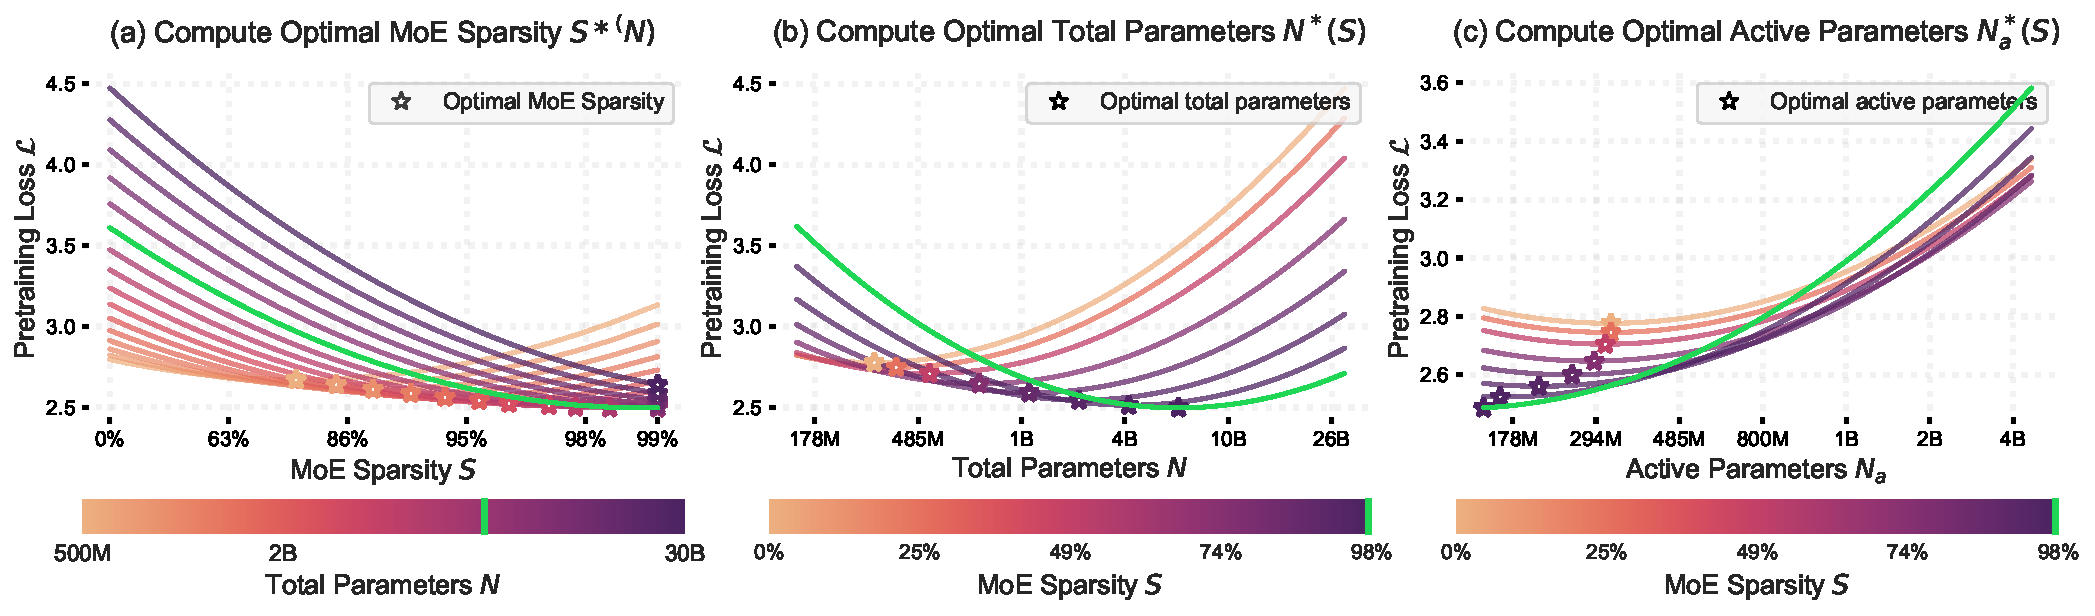
\includegraphics[width=0.45\textwidth]{plots/appendix/app_s2_slices_3e19_fixed_range.pdf}
        \label{fig:slices_3e19}
}    
    \subfigure{
        \centering
        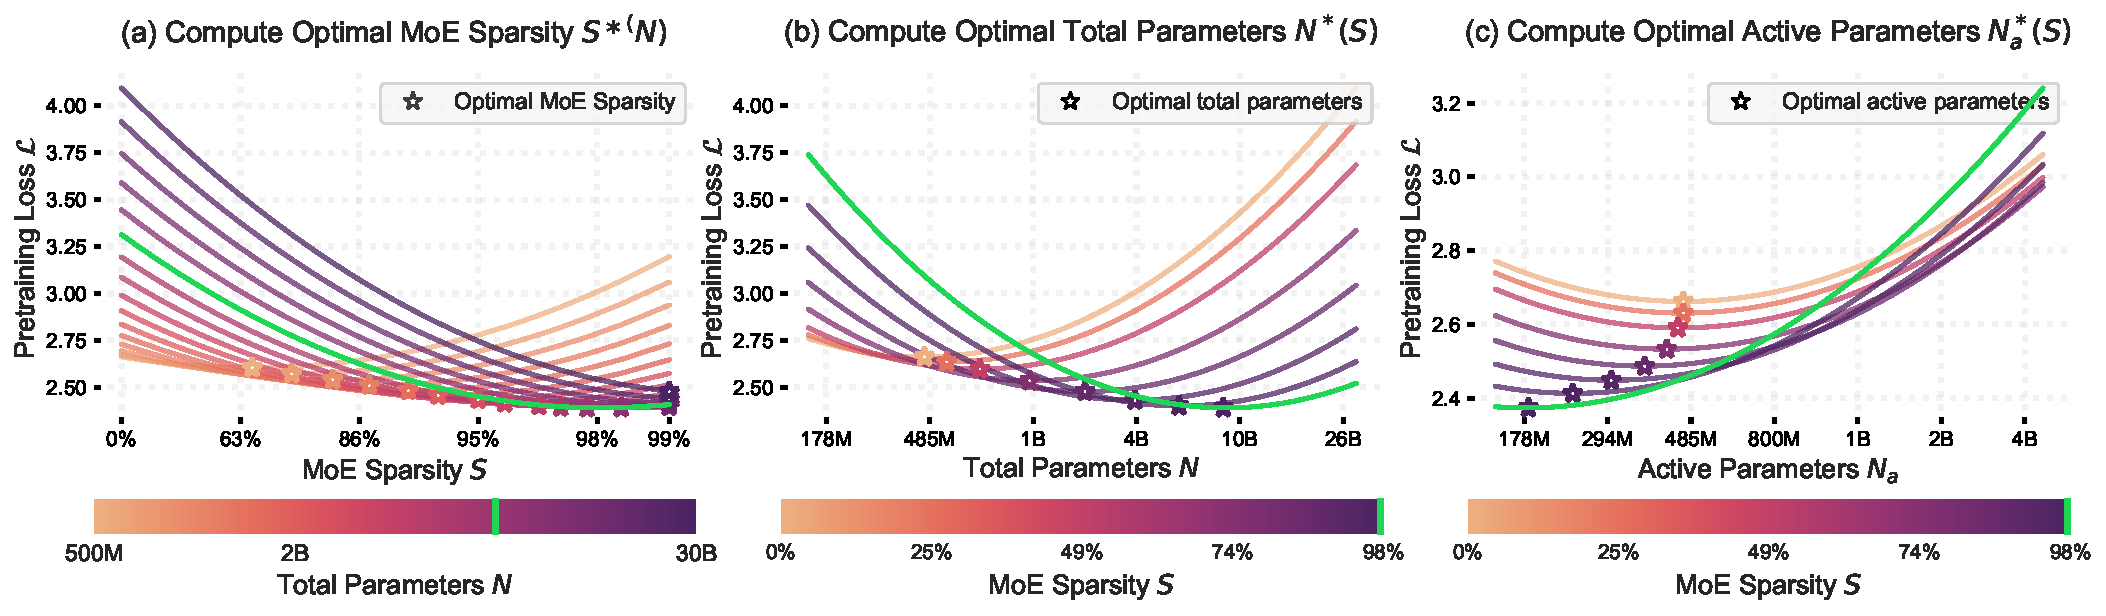
\includegraphics[width=0.45\textwidth]{plots/appendix/app_s2_slices_6e19_fixed_range.pdf}
        \label{fig:slices_6e19}
}
    \subfigure{
        \centering
        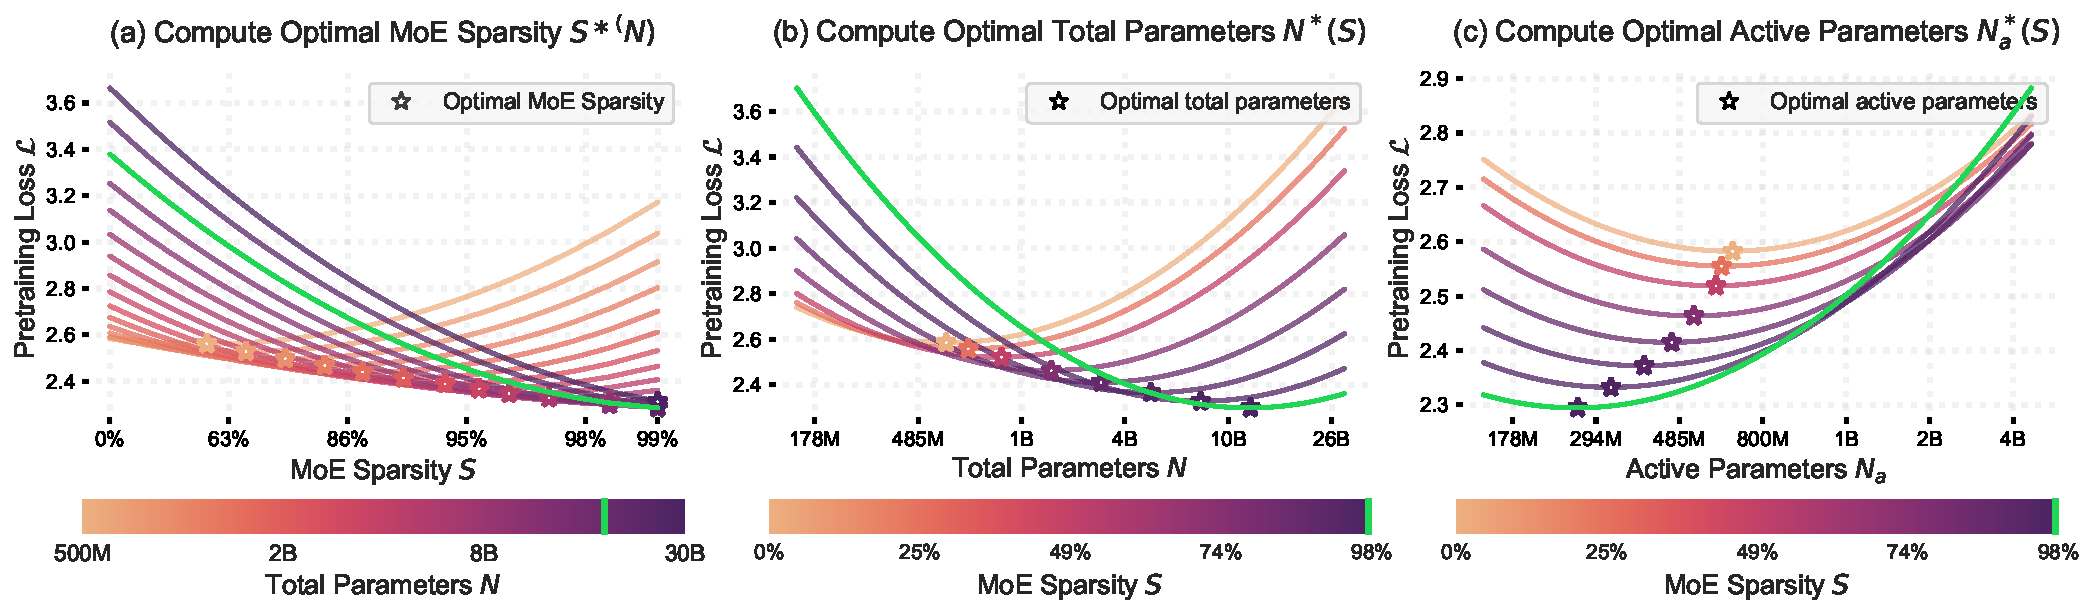
\includegraphics[width=0.45\textwidth]{plots/appendix/app_s2_slices_1e20_fixed_range.pdf}
        \label{fig:slices_1e20}
}
    \subfigure{
        \centering
        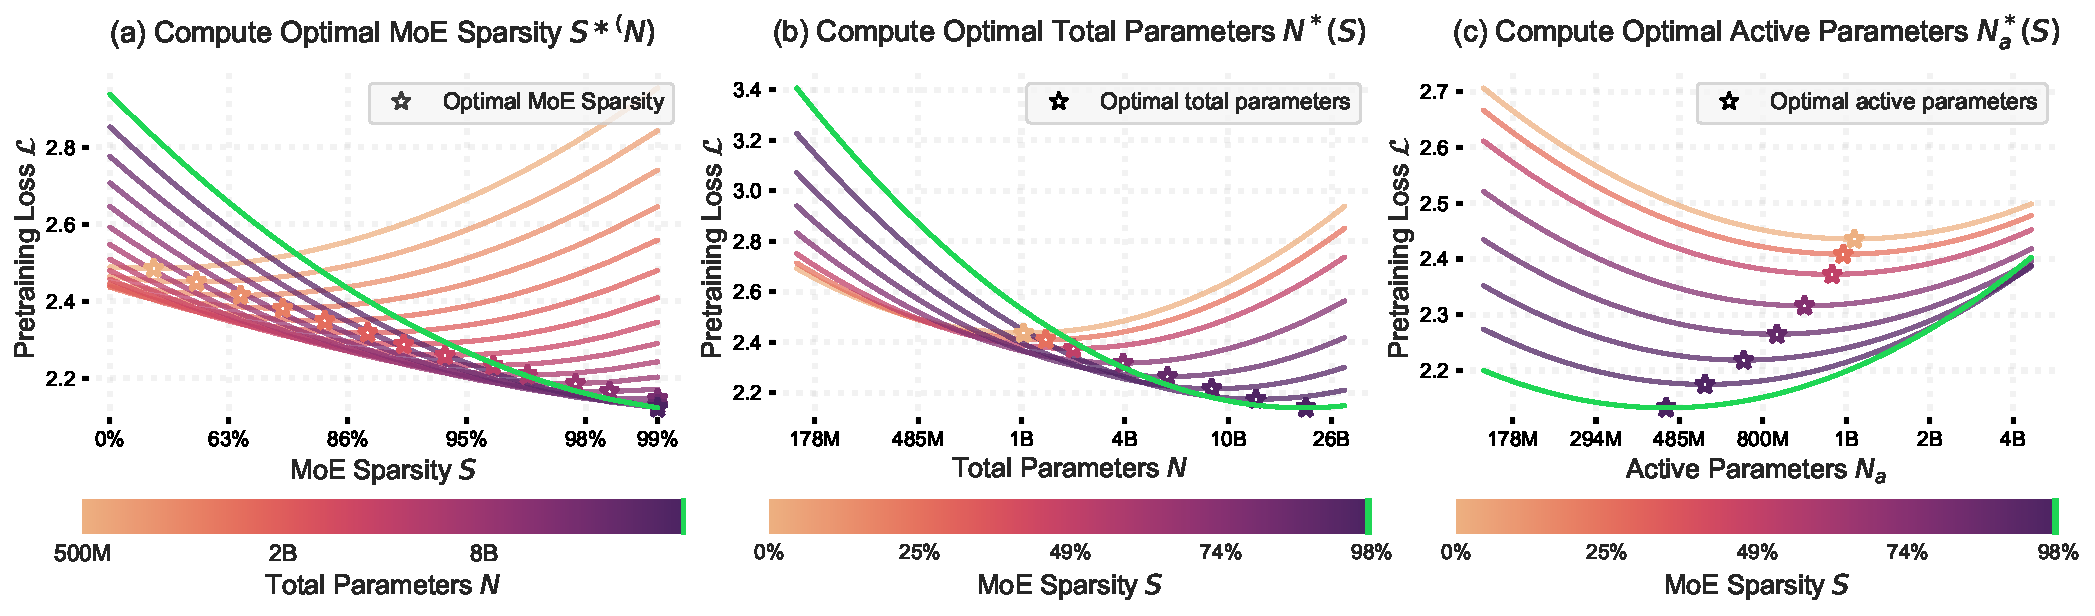
\includegraphics[width=0.45\textwidth]{plots/appendix/app_s2_slices_3e20_fixed_range.pdf}
        \label{fig:slices_3e20}
}    
\subfigure{
        \centering
        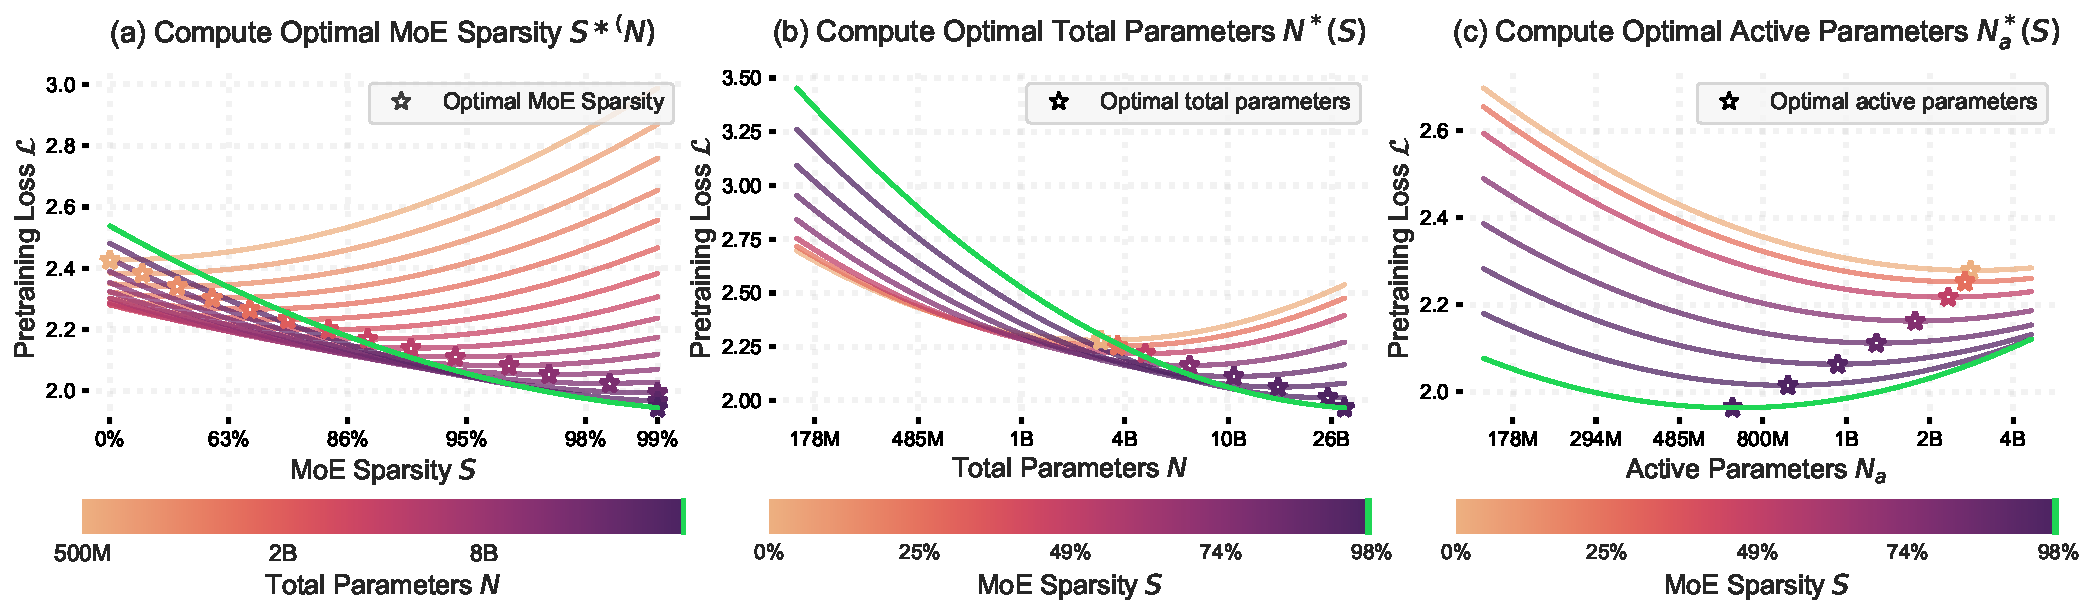
\includegraphics[width=0.45\textwidth]{plots/appendix/app_s2_slices_1e21_fixed_range.pdf}
        \label{fig:slices_1e21}
}
    \caption{
        \textbf{Optimal \moe configurations predictably change with training compute budget.}
        Each row corresponds to an analysis of how optimal \moe sparsity $S^*$, total parameters $N^*$, and active parameters $N^*_a$ change for a given training budget. 
        The subplots on the left show that (a) increasing the training budget increases the model size $N$ (denoted with black dots) with the minimum pretraining loss and (b) for models smaller than a threshold (which increases with training budget), dense models (i.e., $0\%$ sparsity) fare better than sparse \moes. 
        The subplots in the second and third panel show that (a) increasing \moe sparsity increases the optimal total parameters $N^*$ and decreases the optimal active parameters $N^*_a$. In both cases, for a fixed sparsity level, increasing the budget shifts increases the optimal total and active parameters. 
    }
    \label{fig:additional_surface_eval}
\end{figure}

